% author:   sam tenka
% change:   2022-05-18
% create:   2022-05-18

%==============================================================================
%=====  0.  DOCUMENT SETTINGS  ================================================
%==============================================================================

%~~~~~~~~~~~~~~~~~~~~~~~~~~~~~~~~~~~~~~~~~~~~~~~~~~~~~~~~~~~~~~~~~~~~~~~~~~~~~~
%~~~~~~~~~~~~~  0.0. About and Beyond this Exposition  ~~~~~~~~~~~~~~~~~~~~~~~~

%---------------------  0.0.0. page geometry  ---------------------------------
\documentclass[11pt, justified]{tufte-book}
\geometry{
  left           = 0.90in, % left margin
  textwidth      = 4.95in, % main text block
  marginparsep   = 0.15in, % gutter between main text block and margin notes
  marginparwidth = 2.30in, % width of margin notes
                 % 0.20in  % width from margin to edge
}

%---------------------  0.0.1. math packages  ---------------------------------
\newcommand\hmmax{0}
\newcommand\bmmax{0}
\usepackage{amsmath, amssymb, amsthm, mathtools, bm, euler}
\usepackage{listings}
\usepackage{xstring}%hanging, txfonts, ifthen}

%---------------------  0.0.2. graphics packages  -----------------------------
\usepackage{graphicx, xcolor}
\usepackage{enumitem}\setlist{nosep}
\usepackage{float, capt-of}

%~~~~~~~~~~~~~~~~~~~~~~~~~~~~~~~~~~~~~~~~~~~~~~~~~~~~~~~~~~~~~~~~~~~~~~~~~~~~~~
%~~~~~~~~~~~~~  0.1. Header Formatting  ~~~~~~~~~~~~~~~~~~~~~~~~~~~~~~~~~~~~~~~

\definecolor{mgrn}{rgb}{0.15, 0.65, 0.05} \newcommand{\grn}{\color{mgrn}}
\definecolor{mred}{rgb}{0.90, 0.05, 0.05} \newcommand{\red}{\color{mred}}
\definecolor{mbro}{rgb}{0.75, 0.05, 0.05} \newcommand{\bro}{\color{mbro}}
\definecolor{mcya}{rgb}{0.10, 0.45, 0.45} \newcommand{\cya}{\color{mcya}}
\definecolor{mblu}{rgb}{0.05, 0.35, 0.70} \newcommand{\blu}{\color{mblu}}
\definecolor{mbre}{rgb}{0.30, 0.45, 0.60} \newcommand{\bre}{\color{mbre}}
\definecolor{mgre}{rgb}{0.55, 0.55, 0.50} \newcommand{\gre}{\color{mgre}}

\newcommand{\offour}[1]{
    {\tiny \raisebox{0.04cm}{\scalebox{0.9}{$\substack{
        \IfSubStr{#1}{0}{{\blacksquare}}{\square}   
        \IfSubStr{#1}{1}{{\blacksquare}}{\square} \\ 
        \IfSubStr{#1}{2}{{\blacksquare}}{\square}   
        \IfSubStr{#1}{3}{{\blacksquare}}{\square}   
        %\ifthenelse{\equal{#1}{0}}{{\red\blacksquare}}{\square}
        %\ifthenelse{\equal{#1}{1}}{{\red\blacksquare}}{\square} \\ 
        %\ifthenelse{\equal{#1}{2}}{{\red\blacksquare}}{\square}   
        %\ifthenelse{\equal{#1}{3}}{{\red\blacksquare}}{\square}    
    }$}}}%
}



%\newcommand{\note}[1]{{\blu \textsf{#1}}}
\newcommand{\attn}[1]{{\bro \textsf{#1}}}
\newcommand{\attnsam}[1]{{\red $\star$~~\textsf{#1}~~$\star$}}

%---------------------  0.1.0. tidbit headers  --------------------------------
\newcommand{\samtitle} [1]{
  \par\noindent{\Huge \sf \blu #1}
  \vspace{0.4cm}
}

\newcommand{\samquote} [2]{
    \marginnote[-0.4cm]{\begin{flushright}
    \scriptsize
        \gre {\it #1} \\ --- #2
    \end{flushright}}
}

%---------------------  0.1.1. section headers  -------------------------------

\newcommand{\samsection} [1]{
  \vspace{0.5cm}
  \par\noindent{\LARGE \sf \blu #1}
  \vspace{0.1cm}\par
}

\newcommand{\samsubsection}[1]{
  \vspace{0.3cm}
  \par\noindent{\Large \sf \bre #1}
  \vspace{0.1cm}\par
}

\newcommand{\samsubsubsection}[1]{
   \vspace{0.1cm}
   \par\noindent{\hspace{-2cm}\normalsize \sc \gre #1} ---
}

%---------------------  0.1.2. clear the bibliography's header  ---------------
\usepackage{etoolbox}
\patchcmd{\thebibliography}{\section*{\refname}}{}{}{}

%~~~~~~~~~~~~~~~~~~~~~~~~~~~~~~~~~~~~~~~~~~~~~~~~~~~~~~~~~~~~~~~~~~~~~~~~~~~~~~
%~~~~~~~~~~~~~  0.2. Math Symbols and Blocks  ~~~~~~~~~~~~~~~~~~~~~~~~~~~~~~~~~

%---------------------  0.2.0. probability symbols  ---------------------------
\newcommand{\KL}{\text{KL}}
\newcommand{\EN}{\text{H}}
\newcommand{\note}[1]{{\blu \textsf{#1}}}

\newcommand{\scirc}{\mathrel{\mathsmaller{\mathsmaller{\mathsmaller{\circ}}}}}
\newcommand{\cmop}[2]{{(#1\!\to\!#2)}}

% losses averaged in various ways: 
\newcommand{\Ein}  {\text{trn}_{\sS}}
\newcommand{\Einb} {\text{trn}_{\check\sS}}
\newcommand{\Einc} {\text{trn}_{\sS\sqcup \check\sS}}
\newcommand{\Egap} {\text{gap}_{\sS}}
\newcommand{\Eout} {\text{tst}}



%---------------------  0.2.1. double-struck and caligraphic letters  ---------
\newcommand{\Aa}{\mathbb{A}}\newcommand{\aA}{\mathcal{A}}
\newcommand{\Bb}{\mathbb{B}}\newcommand{\bB}{\mathcal{B}}
\newcommand{\Cc}{\mathbb{C}}\newcommand{\cC}{\mathcal{C}}
\newcommand{\Dd}{\mathbb{D}}\newcommand{\dD}{\mathcal{D}}
\newcommand{\Ee}{\mathbb{E}}\newcommand{\eE}{\mathcal{E}}
\newcommand{\Ff}{\mathbb{F}}\newcommand{\fF}{\mathcal{F}}
\newcommand{\Gg}{\mathbb{G}}\newcommand{\gG}{\mathcal{G}}
\newcommand{\Hh}{\mathbb{H}}\newcommand{\hH}{\mathcal{H}}
\newcommand{\Ii}{\mathbb{I}}\newcommand{\iI}{\mathcal{I}}
\newcommand{\Jj}{\mathbb{J}}\newcommand{\jJ}{\mathcal{J}}
\newcommand{\Kk}{\mathbb{K}}\newcommand{\kK}{\mathcal{K}}
\newcommand{\Ll}{\mathbb{L}}\newcommand{\lL}{\mathcal{L}}
\newcommand{\Mm}{\mathbb{M}}\newcommand{\mM}{\mathcal{M}}
\newcommand{\Nn}{\mathbb{N}}\newcommand{\nN}{\mathcal{N}}
\newcommand{\Oo}{\mathbb{O}}\newcommand{\oO}{\mathcal{O}}
\newcommand{\Pp}{\mathbb{P}}\newcommand{\pP}{\mathcal{P}}
\newcommand{\Qq}{\mathbb{Q}}\newcommand{\qQ}{\mathcal{Q}}
\newcommand{\Rr}{\mathbb{R}}\newcommand{\rR}{\mathcal{R}}
\newcommand{\Ss}{\mathbb{S}}\newcommand{\sS}{\mathcal{S}}
\newcommand{\Tt}{\mathbb{T}}\newcommand{\tT}{\mathcal{T}}
\newcommand{\Uu}{\mathbb{U}}\newcommand{\uU}{\mathcal{U}}
\newcommand{\Vv}{\mathbb{V}}\newcommand{\vV}{\mathcal{V}}
\newcommand{\Ww}{\mathbb{W}}\newcommand{\wW}{\mathcal{W}}
\newcommand{\Xx}{\mathbb{X}}\newcommand{\xX}{\mathcal{X}}
\newcommand{\Yy}{\mathbb{Y}}\newcommand{\yY}{\mathcal{Y}}
\newcommand{\Zz}{\mathbb{Z}}\newcommand{\zZ}{\mathcal{Z}}

\newcommand{\sfa}{\mathsf{a}}\newcommand{\fra}{\mathcal{a}}
\newcommand{\sfb}{\mathsf{b}}\newcommand{\frb}{\mathcal{b}}
\newcommand{\sfc}{\mathsf{c}}\newcommand{\frc}{\mathcal{c}}
\newcommand{\sfd}{\mathsf{d}}\newcommand{\frd}{\mathcal{d}}
\newcommand{\sfe}{\mathsf{e}}\newcommand{\fre}{\mathcal{e}}
\newcommand{\sff}{\mathsf{f}}\newcommand{\frf}{\mathcal{f}}
\newcommand{\sfg}{\mathsf{g}}\newcommand{\frg}{\mathcal{g}}
\newcommand{\sfh}{\mathsf{h}}\newcommand{\frh}{\mathcal{h}}
\newcommand{\sfi}{\mathsf{i}}\newcommand{\fri}{\mathcal{i}}
\newcommand{\sfj}{\mathsf{j}}\newcommand{\frj}{\mathcal{j}}
\newcommand{\sfk}{\mathsf{k}}\newcommand{\frk}{\mathcal{k}}
\newcommand{\sfl}{\mathsf{l}}\newcommand{\frl}{\mathcal{l}}
\newcommand{\sfm}{\mathsf{m}}\newcommand{\frm}{\mathcal{m}}
\newcommand{\sfn}{\mathsf{n}}\newcommand{\frn}{\mathcal{n}}
\newcommand{\sfo}{\mathsf{o}}\newcommand{\fro}{\mathcal{o}}
\newcommand{\sfp}{\mathsf{p}}\newcommand{\frp}{\mathcal{p}}
\newcommand{\sfq}{\mathsf{q}}\newcommand{\frq}{\mathcal{q}}
\newcommand{\sfr}{\mathsf{r}}\newcommand{\frr}{\mathcal{r}}
\newcommand{\sfs}{\mathsf{s}}\newcommand{\frs}{\mathcal{s}}
\newcommand{\sft}{\mathsf{t}}\newcommand{\frt}{\mathcal{t}}
\newcommand{\sfu}{\mathsf{u}}\newcommand{\fru}{\mathcal{u}}
\newcommand{\sfv}{\mathsf{v}}\newcommand{\frv}{\mathcal{v}}
\newcommand{\sfw}{\mathsf{w}}\newcommand{\frw}{\mathcal{w}}
\newcommand{\sfx}{\mathsf{x}}\newcommand{\frx}{\mathcal{x}}
\newcommand{\sfy}{\mathsf{y}}\newcommand{\fry}{\mathcal{y}}
\newcommand{\sfz}{\mathsf{z}}\newcommand{\frz}{\mathcal{z}}


      \newcommand{\phdot}{\phantom{.}}

%---------------------  0.2.2. math environments  -----------------------------
\newtheorem*{qst}{Question}
\newtheorem*{thm}{Theorem}
\newtheorem*{lem}{Lemma}
% ...
\theoremstyle{definition}
\newtheorem*{dfn}{Definition}

%~~~~~~~~~~~~~~~~~~~~~~~~~~~~~~~~~~~~~~~~~~~~~~~~~~~~~~~~~~~~~~~~~~~~~~~~~~~~~~
%~~~~~~~~~~~~~  0.3. Section Headers  ~~~~~~~~~~~~~~~~~~~~~~~~~~~~~~~~~~~~~~~~~

%==============================================================================
%=====  1.  PROLOGUE  =========================================================
%==============================================================================

\begin{document}
\samtitle{twelve steps (optional 6.86x notes)}

\marginnote[-0.05cm]{%
  \normalsize
  \textsc{Table of Contents}
  \begin{description}
      \item[overview] \phdot
      \item[frame] \phdot
      \begin{description}
        \item[step A: factorize]
        \item[step B: type and split]
        \item[step C: visualize]
      \end{description}
    \item[model] \phdot
      \begin{description}
        \item[step D: featurize]
        \item[step E: compute more features]
        \item[step F: regularize]
      \end{description}
    \item[train] \phdot
      \begin{description}
        \item[step G: architect]
        \item[step H: gradient-descend]
        \item[step I: model-select]
      \end{description}
    \item[harvest] \phdot
      \begin{description}
        \item[step J: test]
        \item[step K: interpret]
        \item[step L: predict]
      \end{description}
    \item[example: flooding plains]
    \item[example: ancient tables]
    \item[example: pairing flavors]
  \end{description}
  \attnsam{TODO: make clickable}
}

      6.86x is a course on theory.  We will teach you too much: more than you
      need to get your hands dirty doing machine learning and more than you
      need to talk to your machine learning colleagues.  Because of this, some
      students may find themselves itching for some synopsis of practical ML.
      What code might one write day to day --- not for state-of-the-art R\&D,
      but for vanilla machine learning projects?  These notes give a basic
      answer to this question.

      \attn{You do not need to read these notes at all} to get an A in this
      course; conversely, \attn{you may not cite these notes} when solving
      homework or exams.

  %\samsection{0. twelve steps for supervised learning}
      \samsubsubsection{what's inside}
        % PREDICTION
        I'll show you a recipe for learning how to predict outputs from inputs
        based on examples of correct input-output pairs.  That kind of learning
        is called \textbf{supervised learning}.
        %
        In fact, we'll further restrict attention to situations where the
        outputs are of a \textbf{simple type}: \emph{either} 
        they all belong to some known bounded interval (perhaps $[-1, +1]$) of real numbers
        \emph{or}
        they all belong to
        some known finite set.  
        For finite sets I have in mind sets like
        $\{\text{good review}$,  $\text{bad review}$,  $\text{troll review}\}$
        or
        $\{\text{safe}$,  $\text{poisonous}\}$
        or
        $\{\text{black hole}$,  $\text{ordinary star}\}$
        or 
        the set of english words.
        %
        There is technical jargon for the recipe below: it's a recipe for a
        \emph{one-hidden layer leaky-ReLU net with hand-crafted input features
        and with $\ell^1$ regularization determined by hyperparameter search}.
        %
        %I wanted also to discuss \emph{boosted decision trees}.  But I lack time. 
      \samsubsubsection{What's not inside}
        These notes will not help much with developing your understanding
        beyond the blind application of this recipe.  I recommend that you
        go beyond blind application for three reasons:
        \begin{description}
            \item[(a)] these notes neglect important 
                techniques such as boosted decision trees for tabular inputs or 
                convolutional nets for image processing.
                %These are practical techniques that are good to learn.
                The more firmly we're grounded in the 
                %conceptual basis of the
                basics we present here, the more easily we'll assimilate the
                fancy techniques and the more confidently we'll wield them
                in the wild.
            \item[(b)] even when we stick to just the non-fancy techniques in
                 these notes, each bit of rigorous conceptual understanding ---
                 of the \emph{why}, not just the \emph{how} --- will help you
                 impress your intent upon your machine learning models.  For
                 example, if you understand what sparsity has to do with
                 learning and why $\ell^1$ but not $\ell^2$ regularization
                 encourages sparsity, then you'll know when and how to 
                 to invent
                 intermediate regularizations that encourage sparsity along
                 chosen axes.\marginnote{\attnsam{mention EYE REGULARIZATION}}
            \item[(c)] I'm a teacher and an academic; I can't help but hope that y'all dig deeper :-)
        \end{description}

      \samsubsubsection{running examples}
        To illustrate the steps as we describe them, I'll show how they apply
        to two artificially simple examples.

        The first I'll call the \textbf{digits} example: we want to classify a
        photograph of a handwritten digit (gray-scale, $28\times 28$ pixels)
        by what digit it represents.  This will help the post office handle
        all but the messiest writing automatically.

        The second I'll call the \textbf{dances} example: we have a sequence of
        the three-dimensional locations of a dancer's twenty major joints,\marginnote{%
          $\leftarrow$ The twenty joints are (the left and right) 
          bigtoetip, ankle, knee, hip, shoulder, elbow,
          wrist, thumbtip; and the tailbone, mid back bone, atlas neck bone, skulltop. 
        } sampled once every five seconds, and we want to interpolate to eighty
        ``frames'' every five seconds.  This will help our animation team make
        their rough draft.

%~~~~~~~~~~~~~~~~~~~~~~~~~~~~~~~~~~~~~~~~~~~~~~~~~~~~~~~~~~~~~~~~~~~~~~~~~~~~~~
%~~~~~~~~~~~~~  1.x.                                   ~~~~~~~~~~~~~~~~~~~~~~~~

  \newpage
  \samsection{overview}

    \samsubsection{no pytorch}
    
      \samsubsubsection{architecture}
        \begin{lstlisting}[language=Python, basicstyle=\footnotesize\ttfamily]
          #####################################################################

          def featurize(x):
            ...

          #####################################################################

          LEAK = 0.2
          leaky_relu  = lambda z: np.maximum(LEAK*z, z)
          dleaky_relu = lambda z: ((1+0.5*np.sign(z))+LEAK)/(1.0+LEAK)

          def predict(x, A, B):
            f  = featurize(x)     ;   zb = np.matmul(B,f)
            h  = leaky_relu(zb)   ;   za = np.matmul(A,h)
            p  = normalize(np.exp(za))
            return p, (f,zb,h,za,p)

          def acc(y,x, A,B):
            p, _ = predict(x, A, B)
            return 1.0 if y==np.argmax(p) else 0.0  

          #####################################################################

          def loss(y,x, A,B, reg_A,reg_B):
            p, _ = predict(x, A, B)
            return - np.log(p[y])
                   + reg_A * np.sum(np.sum(np.abs(A))) 
                   + reg_B * np.sum(np.sum(np.abs(B))) 

          def grad_loss(y,x, A,B, reg_A,reg_B):
            _, (f, zb, h, za, p) = predict(x, A, B)

            dl_dza = p; dl_dza[y] -= 1.0
            dl_dh  = np.transpose(A) * dl_dza 
            dl_dzb = D_leaky_relu(zb) * dl_dh 

            return ( np.outer(dl_dzb, f) + reg_A * np.sign(A),
                     np.outer(dl_dza, h) + reg_B * np.sign(B)  )
        \end{lstlisting}

      \newpage
      \samsubsubsection{splitting}
        \begin{lstlisting}[language=Python, basicstyle=\footnotesize\ttfamily]
          NB_TOTAL = len(all_samples)

          TEST_IMPRECISION = 0.025 
          DEV_IMPRECISION  = 0.025
          NB_MODELS        = 1000

          NB_TEST = int(2.0/TEST_IMPRECISION**2                        )
          NB_DEV = int(2.0/ DEV_IMPRECISION**2 * np.log(1.0+NB_MODELS))
          NB_TRAIN = TOTAL_SIZE - (TEST_SIZE+DEV_SIZE)

          assert   0<NB_TRAIN, "uh oh!  with {} test samples and {} dev samples we'll have no train samples!".format(NB_TEST, NB_DEV) 
          assert 100<NB_TRAIN, "{} train samples isn't enough for me.".format(NB_TRAIN) 

          tail = all_samples 
          train, tail = tail[:NB_TRAIN], tail[NB_TRAIN:] 
          dev  , tail = tail[:NB_DEV  ], tail[NB_DEV  :] 
          test        = tail[:NB_TEST ]

          print('{} total = {} train + {} dev + {} test'.format(NB_TOTAL, NB_TRAIN, NB_DEV, NB_TEST))
        \end{lstlisting}

      \samsubsubsection{optimization}
        \begin{lstlisting}[language=Python, basicstyle=\footnotesize\ttfamily]
          def optimize_param(H,reg_A,reg_B, T, learn_rate, alpha=0.01):
            A = np.random.laplace(0.0, 1.0/np.sqrt(H), (K,H))
            B = np.random.laplace(0.0, 1.0/np.sqrt(D), (H,D))
            for t in range(T):
              grad_losses = [grad_loss(y,x, A,B, reg_A,reg_B) for y,x in train]
              A -= (learn_rate/(alpha*T + t)) * np.mean([gl[0] for gl in grad_losses])
              B -= (learn_rate/(alpha*T + t)) * np.mean([gl[1] for gl in grad_losses])
            return A,B 

          def optimize_hyper():
            best = {'acc':float('-inf'), 'hyper':None, 'param':None}
            for hyper in hypers_to_try: 
              (H,reg_A,reg_B , T,learn_rate) = hyper 
              A,B = optimize_param()
              acc = np.mean([acc(y,x,A,B) for y,x in dev])
              if acc>best['acc']:
                best = {'acc':float('-inf'), 'hyper':hyper, 'param':(A,B)}
            return best

          def optimize():
            best = optimize_hyper()
            acc, hyper, (A,B) = best['acc'], best['hyper'], best['param']
            acc = np.mean([acc(y,x,A,B) for y,x in test])
        \end{lstlisting}

    \samsubsection{pytorch}
    \samsubsection{}
    \samsubsection{}

%~~~~~~~~~~~~~~~~~~~~~~~~~~~~~~~~~~~~~~~~~~~~~~~~~~~~~~~~~~~~~~~~~~~~~~~~~~~~~~
%~~~~~~~~~~~~~  1.x.                                   ~~~~~~~~~~~~~~~~~~~~~~~~

  \newpage
  \samsection{steps A,B,C: framing}
    \samquote{
      The problem is not the problem.
      The problem is your attitude about the problem.
    }{captain jack sparrow}

    \emph{Framing} is about knowing our data and knowing what problem we want
    it to help solve.
    %\marginnote{%
    %  The quartet of ``frame/model/train/harvest'' is probably not standard
    %  terminology.  They're just words that come to mind as I think about
    %  these steps.  The compulsive part of me wishes there was a five-letter
    %  word for ``harvest.''
    %}
    \samsubsection{step  A: factorize        }
      The first step is to \textbf{factorize}.  That's my short-hand for
      putting a problem into a form we have tools to solve, namely a problem of
      the kind \emph{predict-a-simply-typed-output-from-an-input}.  In many 
      cases, we can skip this step, since our problem is already of the right
      kind.  

      \samsubsubsection{for digits}
      \samsubsubsection{for dances}

      Let me give four examples of what we can do if our original problem
      is not of the right kind. 

      \samsubsubsection{tuples}
        \attnsam{Weight sharing}
      \samsubsubsection{sequences}
        We're trying to predict a \emph{sequence}.  Maybe, for instance, we're
        trying to generate a continuation of a paragraph --- so both the input
        and the output are variable-length sequences of english words.
        %
        Uh oh!  This output is not of a ``simple type''.  What do we do?  Well,
        let's divide each single sentence-continuation problem into a
        collection of simpler problems: can we predict the next word in the
        sentence-so-far given all the preceding words?  If our machine learns
        to solve small problem very well, then repeated application of this
        word-by-word prediction will solve the overall sequence-continuation
        problem.  
        %
        It's this divide-and-conquer style of thinking that leads me to call
        this step ``factorization''.

        Now, here are four things to keep in mind when doing this.

        First, repeated application of a literal next-word predictor would
        yield ever longer sentence continuations.  So we should add a ``STOP
        symbol'' by hand: we regard the output type not as belonging to the set
        of english words, but instead to that set together with an artificial,
        new word, \texttt{STOP}.  Once we generate \texttt{STOP}, we know to
        stop generating new words.

        Second, there is a somewhat analogous (but it turns out less important)
        consideration for the inputs.  We might want to frame the next-word
        prediction problem even more rigidly: instead of predicting the next
        word from all past words, we might want to predict the next word from
        the past, say, five words.  We might do this as a
        crude-but-frequently-adequate\marginnote{%
            This sort of consideration properly belongs to \emph{step D (featurize)}.
            But if we are in sequence-land, we ought to look ahead.
        }
        way to tell the machine to focus on the relationships between nearby
        words.  The upshot is that the machine will be more time-efficient and
        data-efficient during training: it won't have to search through the exponentially
        larger class of patterns involving inter-sentence context
        relationships and it won't get distracted by alluring but spurious
        patterns between how the first word of a sentence on page 6 helps to
        predict the first word of page 86.  The downshot is that there
        \emph{are} inter-sentence context relationships in the real word: page 6
        \emph{does} bear upon page 86, even if weakly and in complicated ways
        that are hard to learn from small datasets.  So when we truncate
        the input to just the past five words, we are retreating in our
        ambition.\marginnote{%
            Note: there are more clever but highly task-dependent tricks that
            can get the best of both worlds.  For example, we might featurize
            the ``prefix'' words before the most recent five words into some
            compressed synopsis --- perhaps by extracting the top ten most
            common content words among that prefix --- and feed those along
            with the most recent five words into the next-word predictor.
        }
        It's a design choice to consider, one that human intuition about the
        problem at hand and trial-and-error can help guide.

        Third, if we do this last-five-words truncation, then we've got to do
        something about the edge case where there are fewer than five words in
        our paragraph so far.  Just as with the STOP symbol, let's ``pad'' the
        input sequence with ``START symbols'' so that if there are only three
        real words so far (Say, \texttt{Sam I am}), what we actually feed into
        the predictor is \texttt{START START Sam I am}.

        Fourth, \attnsam{out-of-sample euler error}

      \samsubsubsection{trees and tagged unions}
        The previous discussion on sequences generalizes to other recursive
        data types.  That's just a fancy name for, ``kinds of things that are
        allowed to contain things of the same kind as parts''.  For example,
        the part of a nonempty sequence after its first element is also a
        sequence.  And the left child of a nonempty tree is also a tree.  Lots
        of modern data is structured like a tree.

        We can factor the problem of generating a (say, binary) tree into the
        problems of: (a) generating a child node given its parental context and
        (b) classifying whether a node should be a leaf or a subtree.  

        (b) is the analogue of the \texttt{STOP} discussion in the passage on
        sequences.  The possibility that the parental context might go up some
        fixed number of generations and be padded is analogous to the
        \texttt{START} discussion.

        Turning away from trees, I want to note that \attnsam{tagged unions (i.e.
        sum types i.e. coproduct types)} fit well into our idea of ``types of
        things belonging to a known finite set.''  Generating a member of a
        tagged union amounts to classifying which tag is appropriate, then
        generating data corresponding to that tag.

      \samsubsubsection{functions or dense arrays}

%~~~~~~~~~~~~~~~~~~~~~~~~~~~~~~~~~~~~~~~~~~~~~~~~~~~~~~~~~~~~~~~~~~~~~~~~~~~~~~
%~~~~~~~~~~~~~  1.x.                                   ~~~~~~~~~~~~~~~~~~~~~~~~

    \newpage
    \samsubsection{step  B :    type and split   }

      \samsubsubsection{typing: NULLS for missing data}


      \samsubsubsection{train-dev-test}
        \attnsam{emphasize random seed RANDOM SEED random seed}
        \attnsam{Explain Why split and roles of the three (including
        visualization)}

        Let's uniformly randomly partition our data into three bins:
        \textbf{train}, \textbf{dev(elopment)}, and \textbf{test}.
        %
        The way this works is that we have a bunch of example input-output
        pairs, say ten thousand.  And we split that number into three numbers
        --- say, eight thousand, one thousand, one thousand --- and assign
        eight thousand pairs to the train bin, a disjoint one thousand to the
        dev bin, and a disjoint one thousand to the test bin.

        A simple way to do this is to shuffle (like a deck of cards\marginnote{%
          $\leftarrow$ use \texttt{np.random.shuffle}
        }) the data, then assign
        the first eight thousand of the shuffled data to train, the next one
        thousand to dev, and the remaining to test.

        Sometimes folks like to shuffle in a less random, more constrained
        way.  For example, if we are doing binary classification (say, of
        good vs bad apples; and say for simplicity that the data we start with
        has equally many of either kind), we might want to make sure that
        exactly half of each bin is good apples.  If we left it up to chance, 
        then the fraction of our eight thousand training examples that are good
        apples would probably be \emph{nearly but not exactly} half.
        %
        There are weak theoretical reasons for not doing this less random
        shuffling.\marginnote{%
          $\leftarrow$ One reason is that when we shuffle less
          randomly, the theoretical statistics that underlies our machine
          learning doesn't exactly apply.  Intuitively, it should \emph{very
          nearly apply}, but we can no longer depend on this with confidence.
          %
          \par Though less-random shuffling has the advantage of
          addressing sampling error in the base rate of good apples, it is
          more principled to get the same advantage a different way: by using a
          train/dev/test split like we suggest.  The latter way is more
          principled because it measures \emph{how sensitive} our model
          is to sampling.   
        }
        But it's your choice.

      \samsubsubsection{choosing portions}
        \attnsam{todo: if extreme class imbalance or cost imbalance, then want
        bigger portions}

        How big should the train, dev, and test sets be?  One way to answer
        this question is to consider how precise you'd like the test score to
        be.  Intuitively, if at the end of the day, you'd like to say something
        like \emph{our confidence interval for this model's performance on
        unseen data drawn from the same distribution as the training data is
        $(A\pm x)\%$}, then you'd want more than $10000/x^2$ many testing
        examples. %\marginnote{%
          %$\leftarrow$
          (That $10000$ comes from squaring the ``$100$'' in ``per-cent'').
        %}
        That's assuming that the testing performance is measured in
        percentage points; if not, then shift and scale until it is before
        applying
        this formula.

        We approach the dev set size similarly but not the same.
        There are two differences between dev set and test set:
        (a) we will change our model based on the dev set, so there is a danger
        of overfitting on the dev set.  
        (b) the precision we ask of our dev performance may differ from the
        precision we ask of our test performance.

        Suppose we know in advance that we will test $M$ many different models
        (perhaps during a hyperparameter search \attnsam{explain what this is})
        during development.  If we want even the least precise of these $M$
        many tests to have $(\pm y)\%$ precision, then we'd want more than
        $\ln(1+M) \cdot 10000/y^2$ dev examples.  It's usually reasonable to
        set $y=x$.

      \samsubsubsection{for digits}
        We have $60000$ total pairs.

        Let's aim for roughly $90\%$ testing accuracy; that seems reasonable
        given my intuitions and experience with digit classification via simple
        models like the ones we will use.  To check whether we succeeded in our
        aim, we will want well less than $\pm 10\%$ imprecision in our testing
        score.  So let's be okay with $\pm 4\%$ imprecision.  $10000/4^2=625$;
        so let's have that be our testing set size.

        Then for the dev set, we want $\pm 4\%$ imprecision and we expect to do
        a hyperparameter search over $5\times 5\times 5\times 5$ many different
        models.  So $\ln(1+5^4) \cdot 10000/4^2 \leq 4325$, so let's have that
        many dev pairs.

        What remains are $55000$ training pairs.

      \samsubsubsection{for dances}


%~~~~~~~~~~~~~~~~~~~~~~~~~~~~~~~~~~~~~~~~~~~~~~~~~~~~~~~~~~~~~~~~~~~~~~~~~~~~~~
%~~~~~~~~~~~~~  1.x.                                   ~~~~~~~~~~~~~~~~~~~~~~~~


    \newpage
    \samsubsection{step  C :    visualize        }
    %

      \samsubsubsection{for digits}
      \samsubsubsection{for dances}


%~~~~~~~~~~~~~~~~~~~~~~~~~~~~~~~~~~~~~~~~~~~~~~~~~~~~~~~~~~~~~~~~~~~~~~~~~~~~~~
%~~~~~~~~~~~~~  1.x.                                   ~~~~~~~~~~~~~~~~~~~~~~~~

  \newpage
  \samsection{steps D,E,F: model}
    \samquote{
      What is the felt experience of cognition at the moment one stands in the
      presence of a beautiful boy or flower or bird?
      ....
      there are attributes that are, without exception,
      present across different objects...
    }{elaine scarry}

    \emph{Modeling} is about presenting our data in a way that is easy to
      digest for the computer.  More precisely, we aim to present the data
      in such a way that the patterns that are easy to find are also intuitively
      likely to be true, useful patterns. 
      %
      This is the key stage where we will inject our
      domain knowledge --- that is, our human experience and intuition (about
      which factors are likely to help with prediction) as aided by the
      previous visualization step.

      This is the stage I'm having the most fun writing.  It's the most
      creative stage.  Steps D,E,F are really aspects of the
      same activity: they are like plucking/slicing, juicing/zesting, and
      filtering/mixing when making lemonade.

    \samsubsection{step D:    featurize        }
      \samsubsubsection{one-hot and quantiles} % and quantile transform
        \marginnote{%
          Jenna Wiens taught me that $5$ --- i.e., \emph{quintiles} --- can
          often work with the sorts of data that human professionals such as
          medical doctors read and write. 
        }
      \samsubsubsection{pretraining and unlabeled side data}
      \samsubsubsection{ideas in signal processing}
        % PID (derivatives, integrals), fourier, masks, etc
        % counting (bag'o'words, ngrams) (Q: WHAT ARE SOME NON-NLP EXAMPLES?) --- view counting as just signal-processing summation with mask? 
      \samsubsubsection{covariant-contravariant} % e.g. coordinates of darkest pixel etc

      \samsubsubsection{for digits}
      \samsubsubsection{for dances}

%~~~~~~~~~~~~~~~~~~~~~~~~~~~~~~~~~~~~~~~~~~~~~~~~~~~~~~~~~~~~~~~~~~~~~~~~~~~~~~
%~~~~~~~~~~~~~  1.x.                                   ~~~~~~~~~~~~~~~~~~~~~~~~

    \newpage
    \samsubsection{step  E :    compute more features}
      \samsubsubsection{nullinears and bilinears} % nullinear == bias term
      \samsubsubsection{distances} % connect to nearest neighbot?
      \samsubsubsection{human experts} % such as nearest neighbor?
      \samsubsubsection{shallow trees} % (random feature subset stumps)
      %

      \samsubsubsection{for digits}
      \samsubsubsection{for dances}


%~~~~~~~~~~~~~~~~~~~~~~~~~~~~~~~~~~~~~~~~~~~~~~~~~~~~~~~~~~~~~~~~~~~~~~~~~~~~~~
%~~~~~~~~~~~~~  1.x.                                   ~~~~~~~~~~~~~~~~~~~~~~~~

    \newpage
    \samsubsection{step  F :    regularize}
      \samsubsubsection{normalization} % for l1 regularization? 
        \marginnote{%
          We'll be using $\ell^1$ regularization for the weights, so the most
          mathematically natural thing is to normalize the $\ell^\infty$ norm
          of each feature.
          %
          Quantile-ization automatically does this.  (caution: still want to
          clip in case train doesn't give full extent of test range).
          %
          \par
          Or we could clip outliers --- say, by (centering and then) rounding
          any $x$ such that $x^4$ is more than $q$ times the
          training-set-average value of $x^4$, to $q$ times that average with
          the appropriate sign.  I'd start by trying $q=3^4/(1+1+1)$.  This
          clips anything $3$ standard deviations or further from a gaussian's
          mean.
        }
      \samsubsubsection{principal components} % should this belong in "compute more features"?
        % sketching?  (random projections?)

      %%  \   
      %%   ) symmetry and weight sharing both partly belong to the "architecture" section...?
      %%  /  
      %%
      \samsubsubsection{symmetry}       %  
        % clay pot metaphor             %  
        % weight sharing                %  
      \samsubsubsection{???} %  
        
    %

      \samsubsubsection{for digits}
      \samsubsubsection{for dances}


%~~~~~~~~~~~~~~~~~~~~~~~~~~~~~~~~~~~~~~~~~~~~~~~~~~~~~~~~~~~~~~~~~~~~~~~~~~~~~~
%~~~~~~~~~~~~~  1.x.                                   ~~~~~~~~~~~~~~~~~~~~~~~~


  \newpage
  \samsection{steps G,H,I: train}
    \emph{Training} is about getting the computer to digest the data we've
    given it.  Under the hood, the computer will try a zillion candidate
    patterns until it hits upon one that explains the examples relatively well.

    \samsubsection{step G :    architect        }
      \samsubsubsection{our shallow neural net} 
        When our output belongs to a known finite set of size $K$, then 
        our hypothesis class $\hH$ consist of functions $f_{A,B}$ defined by
        $$
            f_{A,B} =
            \text{normalize}
            \circ
            \text{map}_{\exp}
            \circ
            A
            \circ
            \text{map}_{\text{leakyReLU}}
            \circ
            B
            \circ
            \text{featurize}
        $$
        Here, $\text{featurize}$ sends raw inputs to feature vectors as
        designed in previous steps.
        %
        Each of the remaining five factors
        ---
        $\text{normalize}$,
        $\text{map}_{\exp}$,
        $A$,
        $\text{map}_{\text{leakyReLU}}$,
        and
        $B$
        ---
        is a function from lists-of-numbers to lists-of-numbers.
        %
        $A,B$ are matrices that act by matrix multiplication.
        %
        $\text{map}_g$ applies $g$ to each element in a list.
        %
        $\text{normalize}$ divides each entry in a list by
        the sum of that list.

        Now, $A$ must be $K \times W$ and $B$ must be $W \times D$, where $K$
        counts the possible outputs, $W$ is the \textbf{hidden dimension}, and
        $D$ counts the features.

        When our output belongs to a bounded interval (say, $[-1,+1]$),
        we replace 
        $\text{normalize} \circ \text{map}_{\exp}$
        by
        \attnsam{FILL IN}

      \samsubsubsection{loss function} % cross entropy, l^1 regression loss
      \samsubsubsection{extracting predictions} 
      \samsubsubsection{pytorch tips} 

      \samsubsubsection{for digits}
      \samsubsubsection{for dances}

%~~~~~~~~~~~~~~~~~~~~~~~~~~~~~~~~~~~~~~~~~~~~~~~~~~~~~~~~~~~~~~~~~~~~~~~~~~~~~~
%~~~~~~~~~~~~~  1.x.                                   ~~~~~~~~~~~~~~~~~~~~~~~~


    \newpage
    \samsubsection{step  H :    gradient-descend }
      \samsubsubsection{initialization}
        \attnsam{non-convexity; symmetry breaking}
        \attnsam{noise normalization}
      \samsubsubsection{gradient step}
        \attnsam{learning rate}
        \attnsam{class imbalance}
      \samsubsubsection{batches, annealing}
      \samsubsubsection{epochs, termination} % implicit regularization?  check quasi-dev for overfit? 
        % herding in case of stuck learning etc

      \samsubsubsection{for digits}
      \samsubsubsection{for dances}



%~~~~~~~~~~~~~~~~~~~~~~~~~~~~~~~~~~~~~~~~~~~~~~~~~~~~~~~~~~~~~~~~~~~~~~~~~~~~~~
%~~~~~~~~~~~~~  1.x.                                   ~~~~~~~~~~~~~~~~~~~~~~~~


    \newpage
    \samsubsection{step  I :    model-select     }
    %
      \samsubsubsection{grid/random/compromise search}
      \samsubsubsection{thinking about model complexity}
        % qualitative remarks on BIC and irrelevant directions
        % Josh's perspective (c.f. PAC-Bayes?): it's about training sensitivity to parameters and how some parameters escape true prior... 
      \samsubsubsection{}
      \samsubsubsection{using generalization bound theory}

      \samsubsubsection{for digits}
      \samsubsubsection{for dances}



%~~~~~~~~~~~~~~~~~~~~~~~~~~~~~~~~~~~~~~~~~~~~~~~~~~~~~~~~~~~~~~~~~~~~~~~~~~~~~~
%~~~~~~~~~~~~~  1.x.                                   ~~~~~~~~~~~~~~~~~~~~~~~~

  \newpage
  \samsection{steps J,K,L: harvest}
    \samquote{
      I am wiser [than he] ... for
      ... he fancies he knows something 
      ... whereas I ... do not fancy I do.
    }{socrates of athens}
    \samquote{
      The theory of probabilities is at bottom nothing but common sense
      reduced to calculus; it enables us to appreciate with exactness
      [what we] feel with a sort of instinct ...
    }{pierre laplace}

    \emph{Harvesting} is about doing stuff with the pattern the computer
      settled on after it tried a zillion candidates.  The main applications
      we'll discuss are deriving insights from the pattern itself (\emph{which
      factors did the computer recognize as most important?})\ and deploying the
      pattern to predict the outputs corresponding to freshly observed inputs.
      %
      Qualifying those two applications is a sense of how well the computer's
      pattern actually models real data.  That's why we also include testing
      in this stage.

    \samsubsection{step J :  test             }
      \samsubsubsection{importance of not data snooping}
      \samsubsubsection{analysis of success/failure areas} % e.g. confusion matrix
      \samsubsubsection{interpreting failure modes}
      \samsubsubsection{triaging the project}

      \samsubsubsection{for digits}
      \samsubsubsection{for dances}


  
%~~~~~~~~~~~~~~~~~~~~~~~~~~~~~~~~~~~~~~~~~~~~~~~~~~~~~~~~~~~~~~~~~~~~~~~~~~~~~~
%~~~~~~~~~~~~~  1.x.                                   ~~~~~~~~~~~~~~~~~~~~~~~~

    \newpage
    \samsubsection{step K :  interpret        }
      \samsubsubsection{reading the weights} % magnitudes and signs.  
        % accuracy vs credibility vs interpretability
        % caution: "cannot diagonalize", i.e. may be n-ary balancing interactions 
      \samsubsubsection{exploring beyond the inputs' typical set}
        % limitations of non-(causal modeling) 
        % limitations of out-of-distribution modeling --- quantify uncertainty
        %       using level curve generalization bounds?
      \samsubsubsection{studying discovered features}
      \samsubsubsection{task-driven dimension reduction and visualization}

      \samsubsubsection{for digits}
      \samsubsubsection{for dances}

%~~~~~~~~~~~~~~~~~~~~~~~~~~~~~~~~~~~~~~~~~~~~~~~~~~~~~~~~~~~~~~~~~~~~~~~~~~~~~~
%~~~~~~~~~~~~~  1.x.                                   ~~~~~~~~~~~~~~~~~~~~~~~~

    \newpage
    \samsubsection{step L :  predict}
      \samsubsubsection{relation between loss function and confidence interval}
      \samsubsubsection{out of distribution prediction}
      \samsubsubsection{pearl, causality, generating ``explanations''}
      \samsubsubsection{making decisions} % expected utility

      \samsubsubsection{for digits}
      \samsubsubsection{for dances}

%==============================================================================
%=====  6.  EXAMPLE PROJECTS  =================================================
%==============================================================================

  \newpage
  %\samsection{F. Three brief example projects}
  %    Now comes a hurried tour of the kinds of analysis these notes discuss.  I
  %    recommend that you \attn{skim} these three example projects without
  %    trying to understand each step.

    \samsection{1. flooding plains}
      \samquote{
        I shall have to accept the fact, I'm afraid, that [their] mind is a
        very thin soil, laid an inch or two deep upon very barren rock.
      }{virginia woolf}

      \samsubsection{visualization  } % featurization
        \begin{figure}[h]
          \centering
          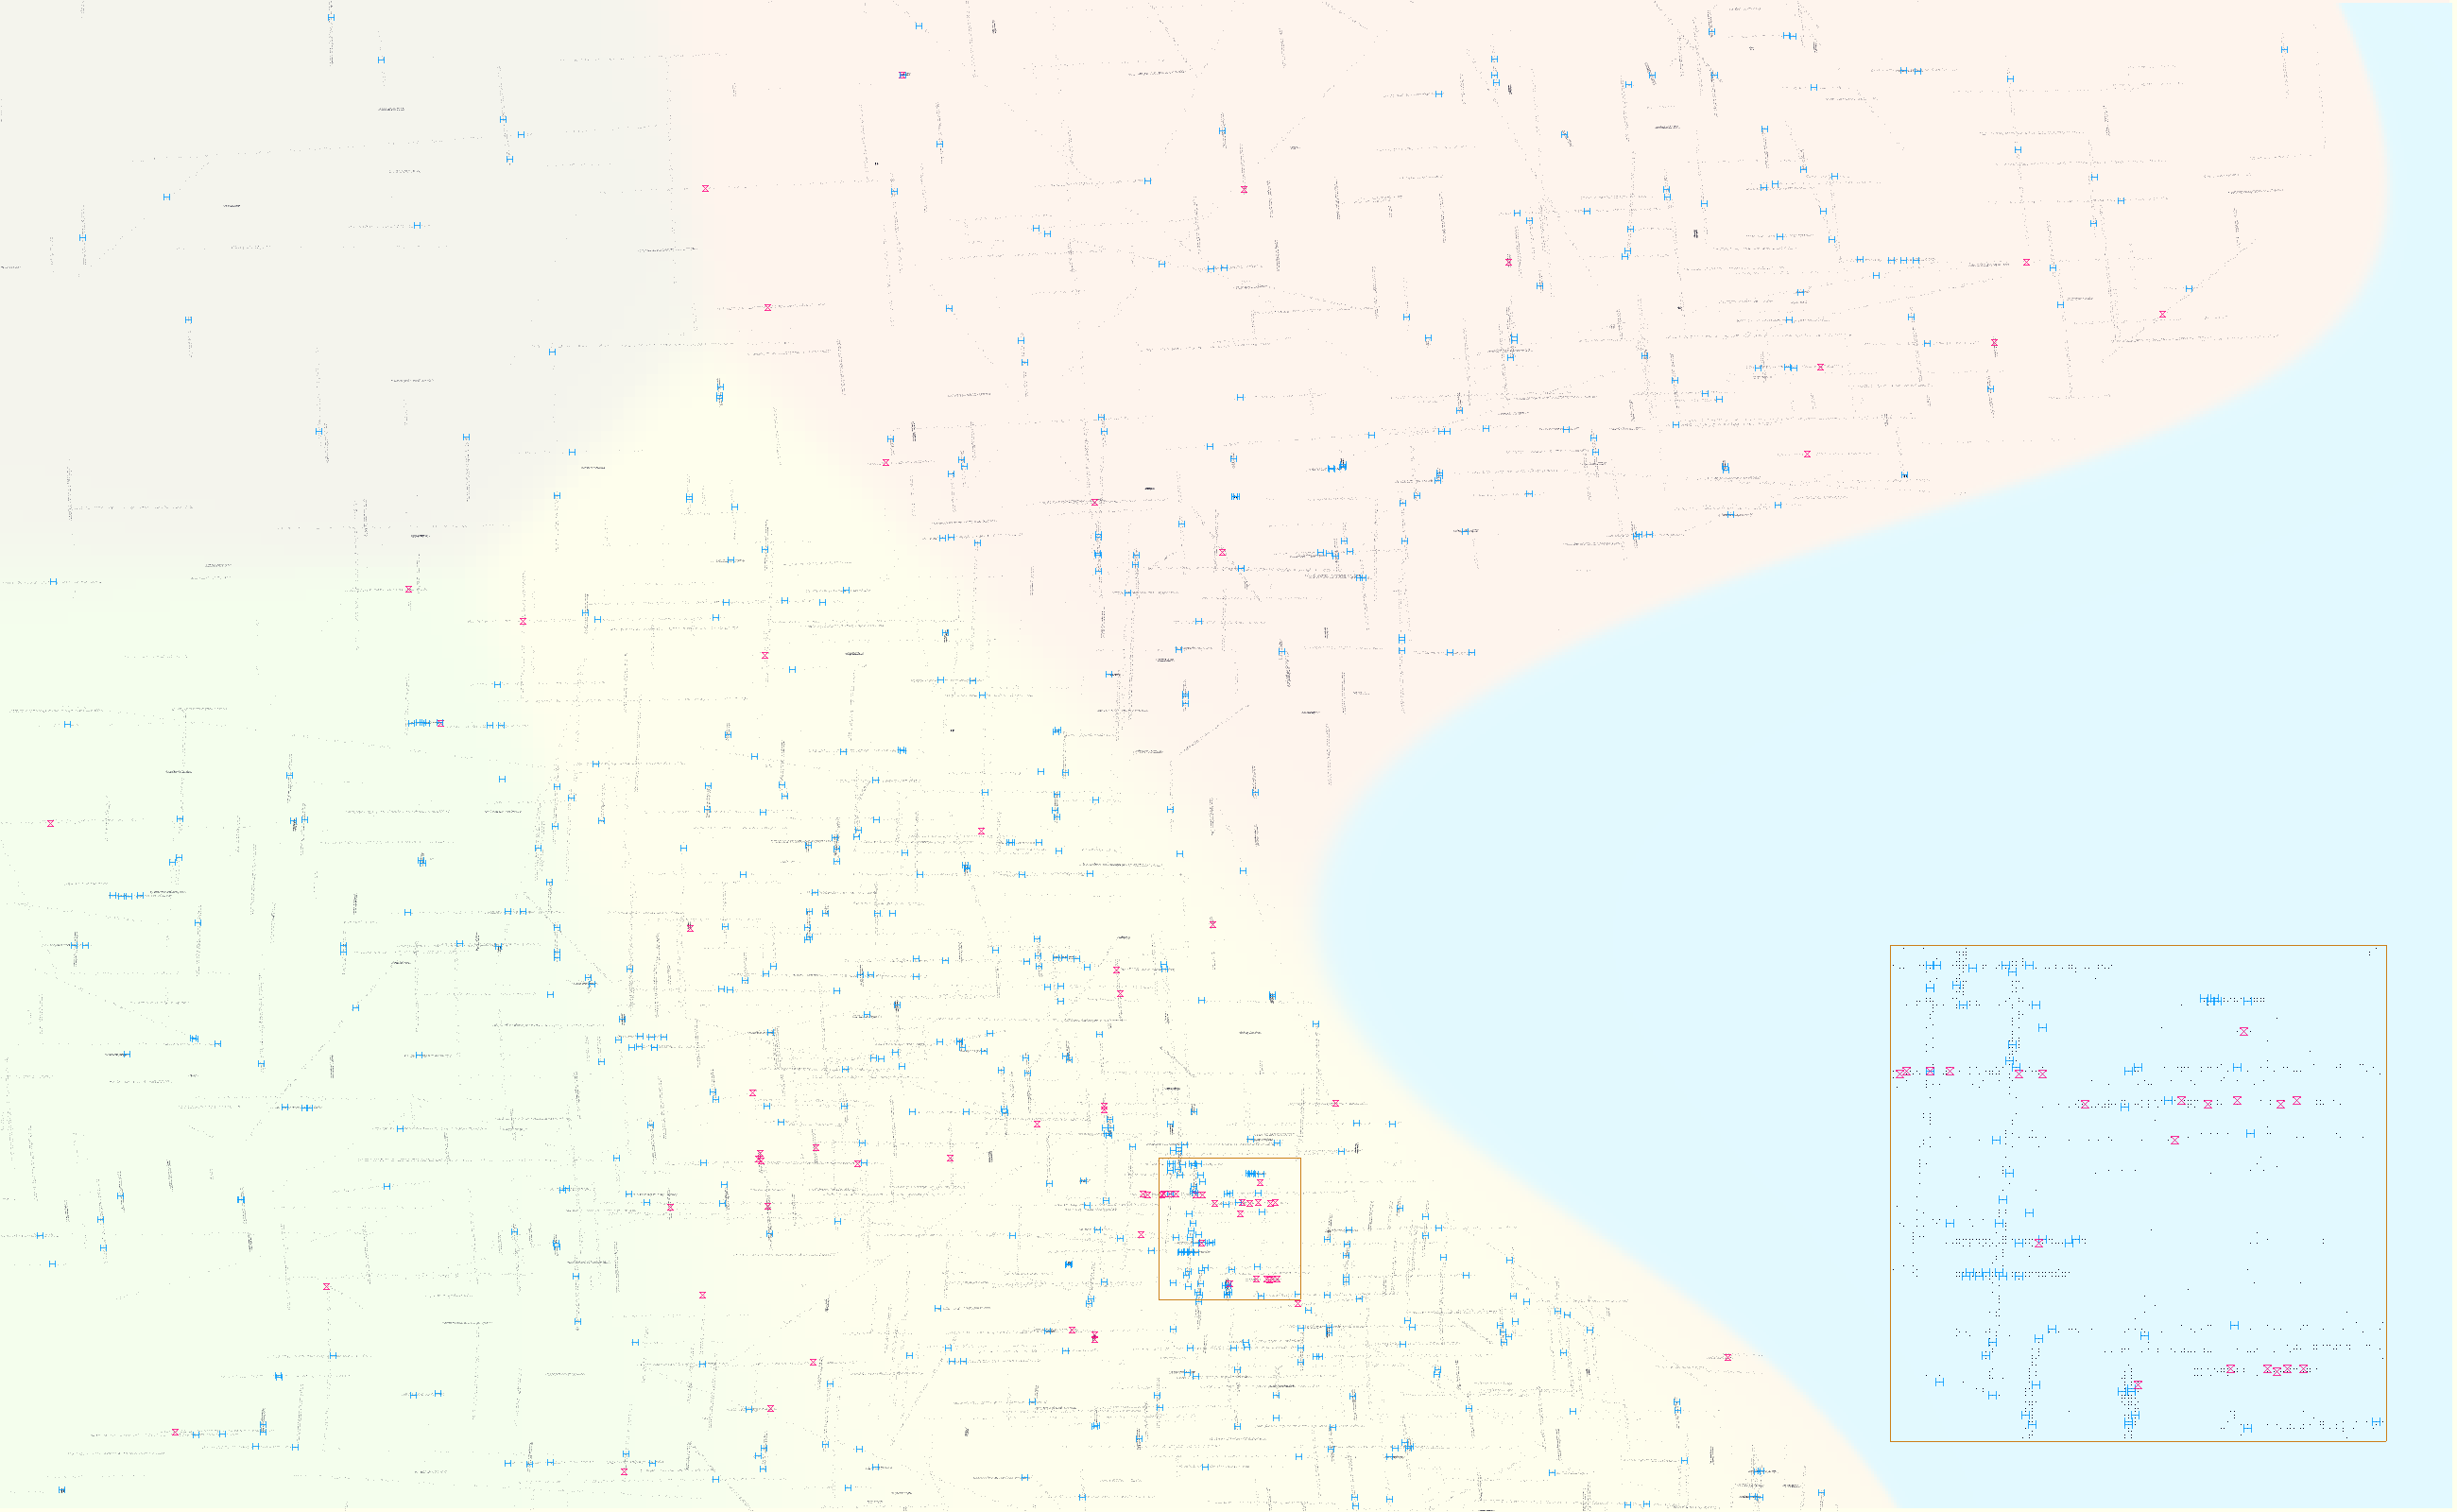
\includegraphics[width=\textwidth]{pipes}
          \captionof{figure}{
            In light yellow and blue are land and sea: $6.4\text{km}\times
            10.4\text{km}$ around the city of Zembla.
            Gray dots:       untested faucets.
            Red bowties:     faucets tested positive.
            Blue I-beams:    faucets tested negative.
            The small yellow box surrounds a neighborhood that enjoyed more
            thorough testing; the large yellow box in the lower right magnifies
            that extra-tested region.
            %
            TODO: number of gray dots, among labels: training set vs hidden 
          }
        \end{figure}


      \samsubsection{fitting        } % featurization
      \samsubsection{model selection} % featurization
      \samsubsection{prediction}
      \samsubsection{overfitting}

      \samsubsubsection{a whimsical story about automation}
        We automate when we re-cast the previous generation's \emph{methods} as
        mere \emph{data} --- data to produce and manipulate. 

        \begin{marginfigure}
            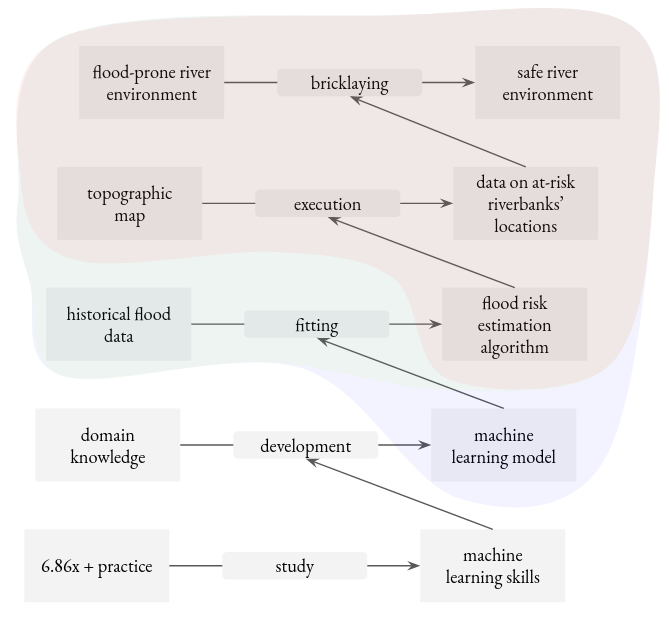
\includegraphics[width=1.0\textwidth]{seven-days}
            \caption{%
              Machine learning continues our human tradition toward the systematic and automatic.
              %
              What for one generation is a luckily discovered idea or recipe
              (bottom tip of red), the next generation refines by
              careful human thought (green). 
              %
              What to one generation is a task (green) requiring human thought
              is to a future generation merely a routine parameterized by some
              newly discovered recipe (bottom tip of blue).
              %
              And the cycle repeats.
              %
              %%\textbf{Left} column: assumed given.
              %%\textbf{Middle} column: activities in the past done by humans and in the future done by machine.
              %%\textbf{Right} column: artifacts valuable either directly (top right corner) or because they help (via diagonal arrows) achieve more direct goals. 
            }
        \end{marginfigure}

        We once sought safety from floods.  Long ago, if we lived near safe
        riverbanks it was by luck; we then found we could make unsafe rivers safe
        by erecting floodwalls.  This was dangerous work, so we built brick
        laying robots to do the hard part.  The machines needed as input some
        flood-risk estimates: the location and mud-softnesses of the river banks to
        work on.

        So we sought flood-risk estimates.  At first, if our city's flood-risk
        estimates were correct it was by luck; we then found we could translate
        topographic maps to flood-risk estimates by applying geology ideas.  This
        was tedious work, so we built computers to do the hard part.  The
        computers needed as input a risk-estimation \emph{algorithm}: a recipe of
        the geology rules to calculate through.

        We thus sought risk-estimation algorithms.  At first, if our research
        center's risk-estimation algorithms were robust to new landscapes it
        was by luck; we then found we could calibrate our algorithms to
        historical flood data from many cities.  To find the better of two
        candidate algorithms, we had to aggregate all their many small success
        and errors.  This was subtle work, so we developed statistical theories
        to do the hard part.  The theories needed as input a \emph{machine
        learning model}: a computationally tractable class of candidate
        algorithms.

        We thus sought machine learning models.  At first, if our machine
        learning models were highly predictive it was by luck; we then found
        general principles to guide model design and selection from domain
        knowledge. % what will we continue to vreate?

        It is these principles that we study in 6.86x.

        Looking back, these are principles that produce machine learning models
        that produce risk-estimation algorithms that produce flood-risk estimates
        that guide the building of floodwalls. 

        \newpage


    \samsection{1. ancient tablets}
      \samquote{
        I am so clever that sometimes I don't understand a single word of what I am saying.
      }{oscar wilde}

      \samsubsection{visualization}
      \samsubsection{transcription}
      \samsubsection{cleaning and imputation}
      \samsubsection{modeling and fitting}
      \samsubsection{generation}
      \samsubsection{a whimsical story about modeling}

    \samsection{2. pairing flavors}
      \samquote{
        Bread that must be sliced with an ax is bread that is too nourishing.
      }{fran lebowitz}

      \samsubsection{visualization}
      \samsubsection{modeling and fitting}
      \samsubsection{regularization}
      \samsubsection{explanation}
      \samsubsection{domain adaptation}
      \samsubsection{a whimsical story about induction}

\end{document}

